\chapter{Implementação}	 
\label{implementacao}
  
  O aplicativo proposto nesse trabalho foi feito utilizando o Android SDK(\textit{Software Development Kit}) que pode ser 
  facilmente obtido em\cite{sdk}, 
  ele foi totalmente escrito em Java e XML. O aplicativo é composto essencialmente por três  classes: MainActivity, 
  Map e WifiInterface. 
  
  A comunicação entre as três classes é feito através da classe Handler\cite{handler} que permite o envio de 
  mensagens entre \textit{threads} e componentes. As principais operações disponíveis no aplicativo não 
  são executadas na \textit{thread} principal, pois, essas operações podem levar muito tempo para serem 
  concluída, assim evitando o problema de travar a execução da \textit{thread} principal, 
  que já foi discutido anteriormente no capitulo sobre Android.
  
  \section{MainActivity}
  A classe MainActivity é responsável por receber as entradas do usuário e exibir os resultados calculados.
  Ela também é responsável por instanciar as duas outras classes. Há três funções disponíveis: 
  \begin{itemize}
   \item \textit{Scan}: Obtém o \textit{fingerprint} da força do sinal wifi dos APs na coordenada informada.
   \item \textit{Save Table}: Salva a tabela de \textit{fingerprints} em um arquivo.
   \item \textit{Get Position}: Obtém a provável posição do aparelho. 
  \end{itemize}

  A MainActivity cria novas \textit{threads} para executar cada uma das operações requerida pelo o usuário.
  
  \section{WifiInterface}
  
  Esta classe centraliza todas as operações envolvendo wifi, como verificar e habilitar a conectividade
  com o wifi do aparelho e obter as informações dos APs(força do sinal, nome do AP, endereço MAC, etc) 
  que estão no alcance do aparelho. Para obter essas informações, o objeto dessa classe
  instancia um BroadcastReceiver que escuta o modulo wifi do aparelho e repassa 
  as informações obtidas através do \textit{Handler} para o componente que requisitou elas.
  
  \section{Map}
  Esta classe é o núcleo da aplicação, ela carrega memória e armazena o mapa de \textit{fingerprints} de RSS que estão 
  guardadas em arquivo. 
  O \textit{fingerprints} é composto 
  pela coordenada informada pelo usuário e as informações obtidas pela classe WifiInterface. 
  Com o mapa de \textit{fingerprints} essa classe executa o algoritmo descrito a seguir para disponibilizar 
  a posição corrente do aparelho.
   
  \section{Algoritmo de Localização baseado em RSS \textit{fingerprinting}}
  
  O algoritmo de localização aqui implementado é dividido em duas etapas: aprendizagem e determinação. Na etapa de aprendizagem, 
  o aplicativo guarda o \textit{fingerprint} dos APs da coordenada informada,
  e salva em uma tabela. O \textit{fingerprint} é composto da média de 8 amostras do RSS de cada AP. A média é utilizada 
  devido a oscilação da força do sinal medido pelo aparelho. O quantidade de \textit{fingerprints} coletados tem um grande 
  impacto na precisão da localização como pode ser observado em \cite{wifiRadar}.  
  
  Na segunda etapa, o processo de localização do aparelho é dividido em três fases. 
  Primeiramente, obtêm-se o \textit{fingerprint} da localidade
  do aparelho com Android, da mesma forma feita na etapa de aprendizagem. 
    
  Na segunda fase, calcula-se a distância Euclidiana, para fazer a comparação com os 
  dados previamente coletados $sqrt((rss1-rss1')^{2}+(rss2-rss2')^{2}+(rss3-rss3')^{2})$, 
e assim encontrar o ponto que mais se aproxima dos parâmetros coletados naquele local, 
 esse processo é repetido para cada conjunto de três APs do \textit{fingerprint}. 
 Assim obtêm-se um conjunto de $n$ pontos que são utilizada na próxima fase. 
  
  A estimativa da posição corrente do aparelho é obtida através do calculo do centroide $C(x_c,y_c)$ desses $n$ pontos:
  \begin{figure}[hbt]
  \centering
  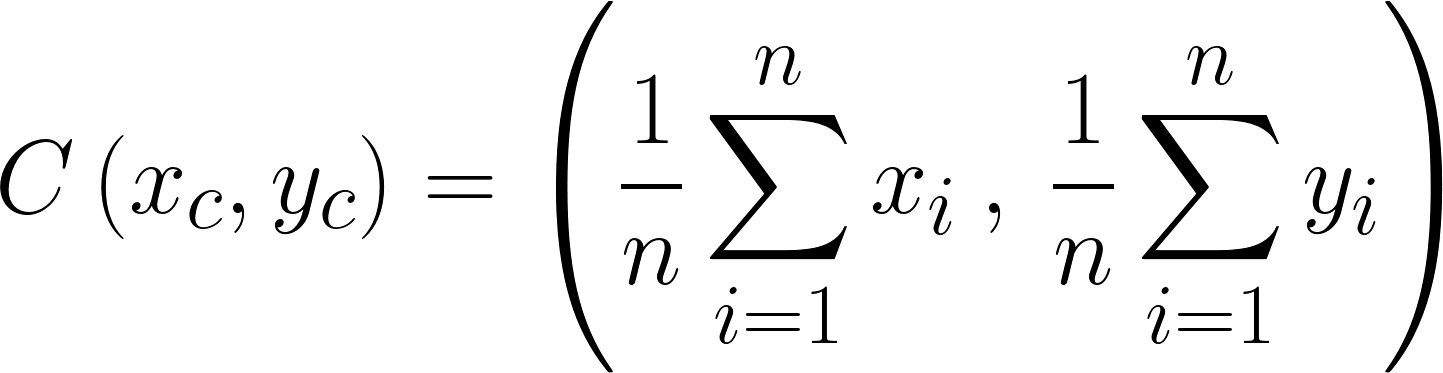
\includegraphics[scale=0.23]{images/centroid.png}
  \caption{Calculo de um centroide de um conjunto de pontos.}
  \label{fig:centroidFormula}
  \end{figure}
  
  $C(x_c,y_c)$ minimiza a soma dos quadrados da distância euclidiana entre ele e os outros $n$ pontos do conjunto\cite{centroid}.
  
      Este algoritmo parte do principio da correlação espacial das localidades adjacentes\cite{fingerPrint2}, 
  que basicamente significa que em uma determinada região do mapa, o RSS dos APs
  mesmo com alterações do ambiente, se mantém com valores similares. Para estimar a posição do aparelho, 
  obtém-se um conjunto de pontos que definem uma região de onde o aparelho possa estar, e a posição final do aparelho 
  e obtida através do centroide desse conjunto de pontos, assim adicionando uma maior robustez 
  a técnica de RSS \textit{fingerprinting}.
  
  \section{Análise e Resultados Obtidos}
  
  As amostras foram obtidos do primeiro andar do departamento de informática da Universidade Federal do Paraná devido a 
  grande quantidade de APs disponíveis(até treze APs em uma coordenada), a imagem abaixo mostra os locais das amostras retiradas.
  Os testes foram executados em um \textit{smartphone} LG Nexus 4, com Android KitKat 4.4.4. 
  -Foram obtidos 67 \textit{fingerprints} de diferentes coordenadas.
  -Foram realizados 35 testes.
  
  
   \begin{figure}[hbt]
  \centering
  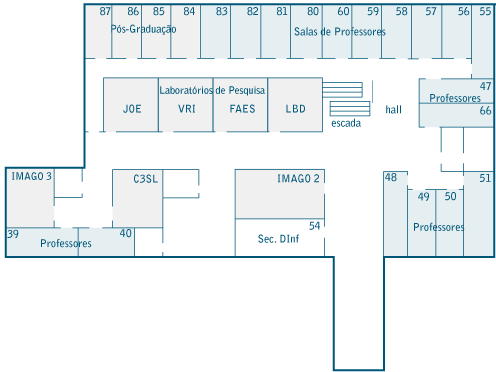
\includegraphics[scale=0.9]{images/mapadinf_andar1_492x327.png}
  \caption{Mapa do primeiro andar do Departamento de Informática da UFPR.}
  \label{fig:mapaDinf}
  \end{figure}
     \clearpage
     \subsection{Resultados Obtidos}
     
     \begin{table}[h]
	  \resizebox{0.8\textwidth}{!}{\begin{minipage}{\textwidth}
         \begin{tabular}{| c | c | c | p{3cm} |}
	    \hline
	    Teste  & Estimativa(x,y) & Real(x,y) & Erro(metros) \\ \hline
	    1 & (4,0) & (4,2) & 2 \\ \hline
	    2 & (4,0) & (4,3) & 3 \\ \hline
	    3 & (6,0) & (7,1) & 1.41 \\ \hline
	    4 & (9,3) & (8,5) & 2.24 \\ \hline
	    5 & (9,8) & (9,9) & 1 \\ \hline
	    6 & (9,9) & (9,11) & 2 \\ \hline
	    7 & (9,10) & (10,8) & 2.24 \\ \hline
	    8 & (9,12) & (9,12) & 0 \\ \hline
	    9 & (9,13) & (7,11) & 2.83 \\ \hline
	    10 & (10,14) & (9,14) & 1 \\ \hline
	    11 & (11,15) & (12,16) & 1.41 \\ \hline
	    12 & (11,15) & (10,15) & 1 \\ \hline
	    13 & (12,15) & (12,15) & 0 \\ \hline	    
	    14 & (14,15) & (12,13) & 2.83 \\ \hline
	    15 & (9,16) & (9,14) & 2 \\ \hline
	    16 & (9,18) & (11,20) & 2.83 \\ \hline
	    17 & (8,20) & (10,19) & 2.24 \\ \hline
	    18 & (10,19) & (9,19) & 1 \\ \hline
	    19 & (7,18) & (8,18) & 1 \\ \hline
	    20 & (6,17) & (7,18) & 1.41 \\ \hline
	    21 & (6,19) & (7,18) & 1.41 \\ \hline
	    22 & (6,19) & (5,17) & 1 \\ \hline
	    23& (4,19) & (5,16) & 2.24 \\ \hline
	    24 & (4,21) & (4,21) & 0 \\ \hline
	    25 & (4,15) & (5,16) & 1.41 \\ \hline
	    26 & (4,11) & (9,12) & 5.1 \\ \hline
	    27 & (4,9) & (5,12) & 3.2 \\ \hline
	    28 & (4,6) & (5,8) & 2.24 \\ \hline
	    29 & (4,3) & (7,8) & 5.83 \\ \hline
	    30 & (4,2) & (5,3) & 1.41 \\ \hline
	    31 & (5,0) & (7,1) & 2.24 \\ \hline
	    32 & (9,1) & (6,5) & 5 \\ \hline
	    33 & (9,7) & (7,9) & 2.83 \\ \hline
	    34 & (9,7) & (7,9) & 2.83 \\ \hline 
	    35 & (9,5) & (7,8) & 3.6 \\ \hline 
	 \end{tabular}
	 \caption[Table caption text]{Tabela com os  resultados obtidos. }
	 \label{table:name}
	 
	\end{minipage} }
     \end{table}
     
    -1m - 25,7 \%
    -3 - 85,7 \%
    -5 - 91,4 \%
    \begin{comment}
  -Criação da tabela:
    -para a coordenada em questão são obtidas 8 amostras da força do sinal wifi, e é feita a 
    média de cada força de sinal wifi de cada AP.
	- Pois O RSS varia muito(exibir exemplo).
  -Calculo da posição(3 fases):
    - Permite obter a posição do aparelho mesmo sem um fingerprint da posição do aparelho.
	- com as triangulações obtem-se o pontos que se aproxima da posição real.
    -obtem se 8 amostras do APs wifis e faz-se média.
    - para cada 3 APs obtem-se um ponto do mapa.
	- Esse ponto é obtido calculando a menor distância euclidiana entre os APs na amostragem e 
	e os dados salvos na tabela.
    - Com o esse conjunto de pontos, calcula-se o mmq com a biblioteca do apache(citar).
      -Onde obtem se o melhor ponto que resume os pontos obtidos.
    -Colocar imagem.
    \end{comment}
  
\begin{comment}
  Os experimentos serão realizados no departamento de informática da Universidade Federal do Paraná, 
  devido a grande quantidade de Access Points disponíveis e a disponibilidade da planta do departamento. 
  A implementação do sistema de navegação será dividida em duas etapas:
  \subsection{Etapa 1}
  
  Uma aplicação escrita em C será utilizada para criação do mapa topológico do departamento. Essa aplicação recebe como entrada:
  \begin{itemize}
    \item Uma imagem contendo o mapa.
    \item Tamanho da célula.
  \end{itemize}
 
  A imagem será dividida em células. Em todas as células, serão aplicadas a função de transformação de Hough \cite{openCV}, da biblioteca OpenCV para detecção de linhas. 
  Esta aplicação devolve uma matriz, onde célula possui uma valor que indica o grau de incerteza de haver um obstáculo: 0 (sem obstáculo) ou 4(com obstaculo). 
  Essa matriz será embarcada na aplicação Android da etapa 2.
  
  O tamanho ideal da célula, será definido via experimentos. Em \cite{cnn} o tamanho da célula tem o tamanho do robô. O artigo \cite{dlite} sugere que o tamanho da célula deve 
  comportar todo o obstáculo, lembrando que a quantidade de células pode influênciar no tempo de processamento do planejamento da trajetória do robô \cite{voronoi}.
  
    Uma segunda aplicação Android, será utilizada para coletar amostras, como descrito no método empírico do artigo\cite{wifiRadar}. As tabelas resultantes dessa aplicaçao, também serão 
  embarcada na aplicação Android da etapa 2. As linha da tabela conterão as coordenadas, RSS e nome do AP da amostra daquele local. Vale ressaltar, que número de amostras tem grande impácto 
  na precisão do calculo da localização \cite{wifiRadar}.
  
  \subsection{Etapa 2}
	A aplicação Android dessa etapa, possui 2 componentes principais: uma \textit{Acitivity} \cite{activity} que fará a interação com o usuário, 
	e um Service \cite{service} que fará o processo de navegação do robô. O robô e o tablet, se comunicarão via \textit{bluetooth},
	ou seja, para o funcionamento do sistema, o tablet deve estar pareado com o robô.

	A \textit{Acitivity} irá obter a posição do clique em relação à imagem do mapa, e obter as coordenadas da posição de destino
	 do robô e repassar para o Service. O usuário deve clicar no botão conectar para que a aplicação possa iniciar uma conexão \textit{bluetooth} com o robô.
	Haverá uma imagem com o mapa do ambiente, o usuário deve apontar o local no qual o robô deve atingir. E então clicar no botão iniciar.
	
	Um Service será iniciado, e executará os seguintes passos:
	\begin{itemize}
	  \item O mapa topológico será carregado na memória.
	  \item A posição do robô será calculada, medindo o RSS\cite{wifiRss} dos APs e aplicando o método descrito em \cite{wifiRadar}.
	  \item Em seguida será aplicado o algoritmo A*\cite{aestrela} na matriz gerada na etapa 1. A função h (heurística) levará em consideração o valor da 
	célula(celulas com valor inferior a 3 serão descartados do caminho) e a sua distância euclidiana, em relação a célula destino. 
	  \item Com o trajeto definido, um comando(vetor de bytes indicando distância e direção) será enviado ao robô.
	  \item O Service aguarda o recebimento dos dados do robô.
	  \item Se nenhum obstáculo é encontrado um novo comando é enviado, e processo se repete, até que o robô atinja seu objetivo.
	  \item Se o robô encontrar um novo obstáculo, a célula onde este foi encontrado é incrementado em 1. 
	  Então o processo de descoberta de trajeto é iniciado novamente.
	  \item Se por acaso o robô verificar está célula de novo e não houver obstáculo, o valor da célula é decrementado em 1.
	  \item Se o robô ficar preso, então é adotado um procedimento descrito em \cite{dlite},
	  muros virtuais são criado, para que o robô evite este caminho em uma segunda passagem.
	\end{itemize}
	
	 Aplicação Arduino faz a interface com os motores, o sonar e o adaptator \textit{bluetooth}.
	 Basicamente, ela executa o comando recebido, e então envia os dados coletados pelo sonar e aguarda um novo comando.
\end{comment}